\section{Durchführung}
\label{sec:Durchführung}
Zu Beginn werden die geometrischen Abmessungen der Platinen für zwei Proben erfasst.
Mit dem Aufbau wie in Abbildung \ref{fig:widerstand} wird der Spannungsabfall am Potentiometer in Abhängigkeit eines Stromes gemessen, daraus kann
der Widerstaand bestimmt werden. Dies wird mit beiden Proben wiederholt.
\begin{figure}
  \centering
  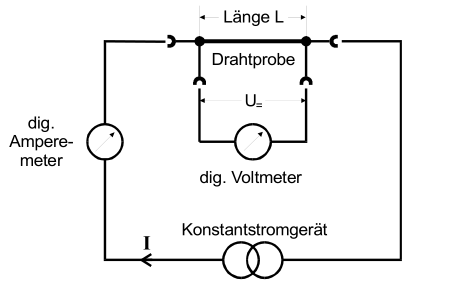
\includegraphics[width=0.5\textwidth]{widerstand.PNG}
  \caption{Aufbaau zur Bestimmung des Widerstandes}
  \label{fig:widerstang}
\end{figure}
Anschließend wird eine Hysteresekurve aufgenommen, dazu wird mit einer Hall-Sonde die magnetische Flussdichte in Abhängigkeit
eines fallenden und eines steigenden Stromes gemessen.
Zuletzt wird die Hall-Spannung an den beiden Proben in Abhängigkeit eines Stromes gemessen.
